\documentclass{article}
\usepackage[utf8]{inputenc}
\usepackage[spanish]{babel}
\usepackage{listings}
\usepackage{graphicx}
\graphicspath{ {images/} }
\usepackage{cite}
\usepackage{url}


\begin{document}

\begin{titlepage}
    \begin{center}
        \vspace*{1cm}
            
        \Huge
        \textbf{Taller de memoria}
            
        \vspace{0.5cm}
        \LARGE
        Nociones de la memoria del computador
            
        \vspace{1.5cm}
            
        \textbf{Sebastián Florez Rios}
            
        \vfill
        
\includegraphics[]{download.jpg}
        
            
        \Large
        Despartamento de Ingeniería Electrónica y Telecomunicaciones\\
        Universidad de Antioquia\\
        Seccional Oriente\\
        Septiembre de 2020
            
    \end{center}
\end{titlepage}

\tableofcontents

\section{Sección introductoria}
Para entender el funcionamiento de un computador, es necesario saber como está compuesto y tener la noción de como funciona cada uno de sus componentes. Este taller se centrará en la memoria, se definirá que es y su uso, tambien conoceremos algunos tipos de memorias. Luego se aondará un poco mas en el tema, conociendo como se gestiona la memoria en un pc y que factores llevan a que una memoria sea mas rápida que otra.    
\section{Desarrollo del taller} \label{contenido}

\textbf{1. Defina que es la memoria del computador.}\vspace{0.5cm} \\

    La memoria de un computador es la encargada de almacenar temporalmente datos que el procesador necesita para realizar procesos inmediatos. Esta parte del hadware es vital para el correcto funcionamiento de la máquina; ya que provee de informaciom indispensable al chip de forma casi instantánea. \vspace{0.5cm} \\
    
\textbf{2. Mencione los tipos de memoria que conoce y haga una pequeña descripción de cada tipo.}\vspace{0.5cm} \\

\textbf{Memoria Ram (Random Access Memory):} Es la memoria mas importante de un pc,almacena diferentes tipos de datos, pero al ser una memoria volatil, no se guardan de forma permanete. Existen diferentes tipos de memoria Ram como la SRAM, SDRAM,RDRAM; varian principalmente en la velocidad de acceso de la información.\vspace{0.5cm} \\

\textbf{Memoria Rom (Read Only Memory):} Es una memoria de solo lectura y es la encargada de dar inicio a la Bios.\vspace{0.5cm} \\

\textbf{Memoria Caché:} Es la encargada de guardar diferentes direcciones de memoria que luego son utilizadas por la Ram para realizar diferentes funciones.\vspace{0.5cm} \\

\textbf{Memoria dedicada:} Tambien se le conoce como tarjeta gráfica y es la encargada de mostrar imágenes en la pantalla, además, ayuda al procesador a trabajar con vídeo, fotografías e imágenes en 3D, entre otras. Este tipo de memoria no es indispensabe para el funcionamiendo del computador. \vspace{0.5cm} \\

\textbf{Disco duro:} Guarda programas y datos del computador. Al no ser volatil, a diferencia de los demas tipos de memoria nombrados, almacena de forma permanente la información, asi el pc esté apagado. \vspace{0.5cm} \\

\textbf{3. Describa la manera como se gestiona la memoria de un computador.}\vspace{0.5cm} \\


Inicialmente por ejemplo el procesador ejecuta un programa y envia una orden a la memoria para que reserve un espacio en ella y así guardar datos de la ejecución del mismo, leyendo por partes la informacion almacenada. Luego de tener el programa en funcionamiento, el micro chip genera nuevos espacios en memoria para el funcionamiento del programa, pero tambien va eliminando otros espacios ocupados y así poder ser utilizados en procesos posteriores. Finalmente al ser finalizado el programa, se eliminan los espacios de memoria utilizados en el programa, para que no ocupen memoria innecesariamente.\vspace{0.5cm} \\

<<La parte del sistema operativo que administra la memoria se llama administrador de memoria y su labor consiste en llevar un registro de las partes de memoria que se estén utilizando y aquellas que no, con el fin de asignar espacio en memoria a los procesos cuando éstos la necesiten y liberándola cuando terminen.>> 1 \vspace{0.5cm} \\

\textbf{4.¿Que hace que una memoria sea mas rápida que otra?¿por qué esto es importante?.} \vspace{0.5cm} \\

Varios factores influyen en la diferencia de velocidad de los diferentes tipos de memoria. Por ejemplo el disco duro HDD es el mas lento de las memorias de un computador, al ser mecanico, busca la información en orden, por lo contrario la memoria Ram no hace esto, puede ir directamente a lo que se necesita. Pero en este orden, la memoria caché se encuentra por encima de la Ram, al estar dentro del microprocesador, asegura un acceso directo del mismo, garantizando así altas velocidades de lectura y almacenamiento. \vspace{2cm} \\ 



\section{Conclusión} \label{conclulsion}

Al conocer las funciones de la memoria, los diferentes tipos y la importancia de la misma, se puede concluir que es vital para el funcionamiento de un computador, así mismo se debe gestionar adecuadamente para su correcto uso, logrando un correcto desempeño de la pc. \vspace{2cm} \\

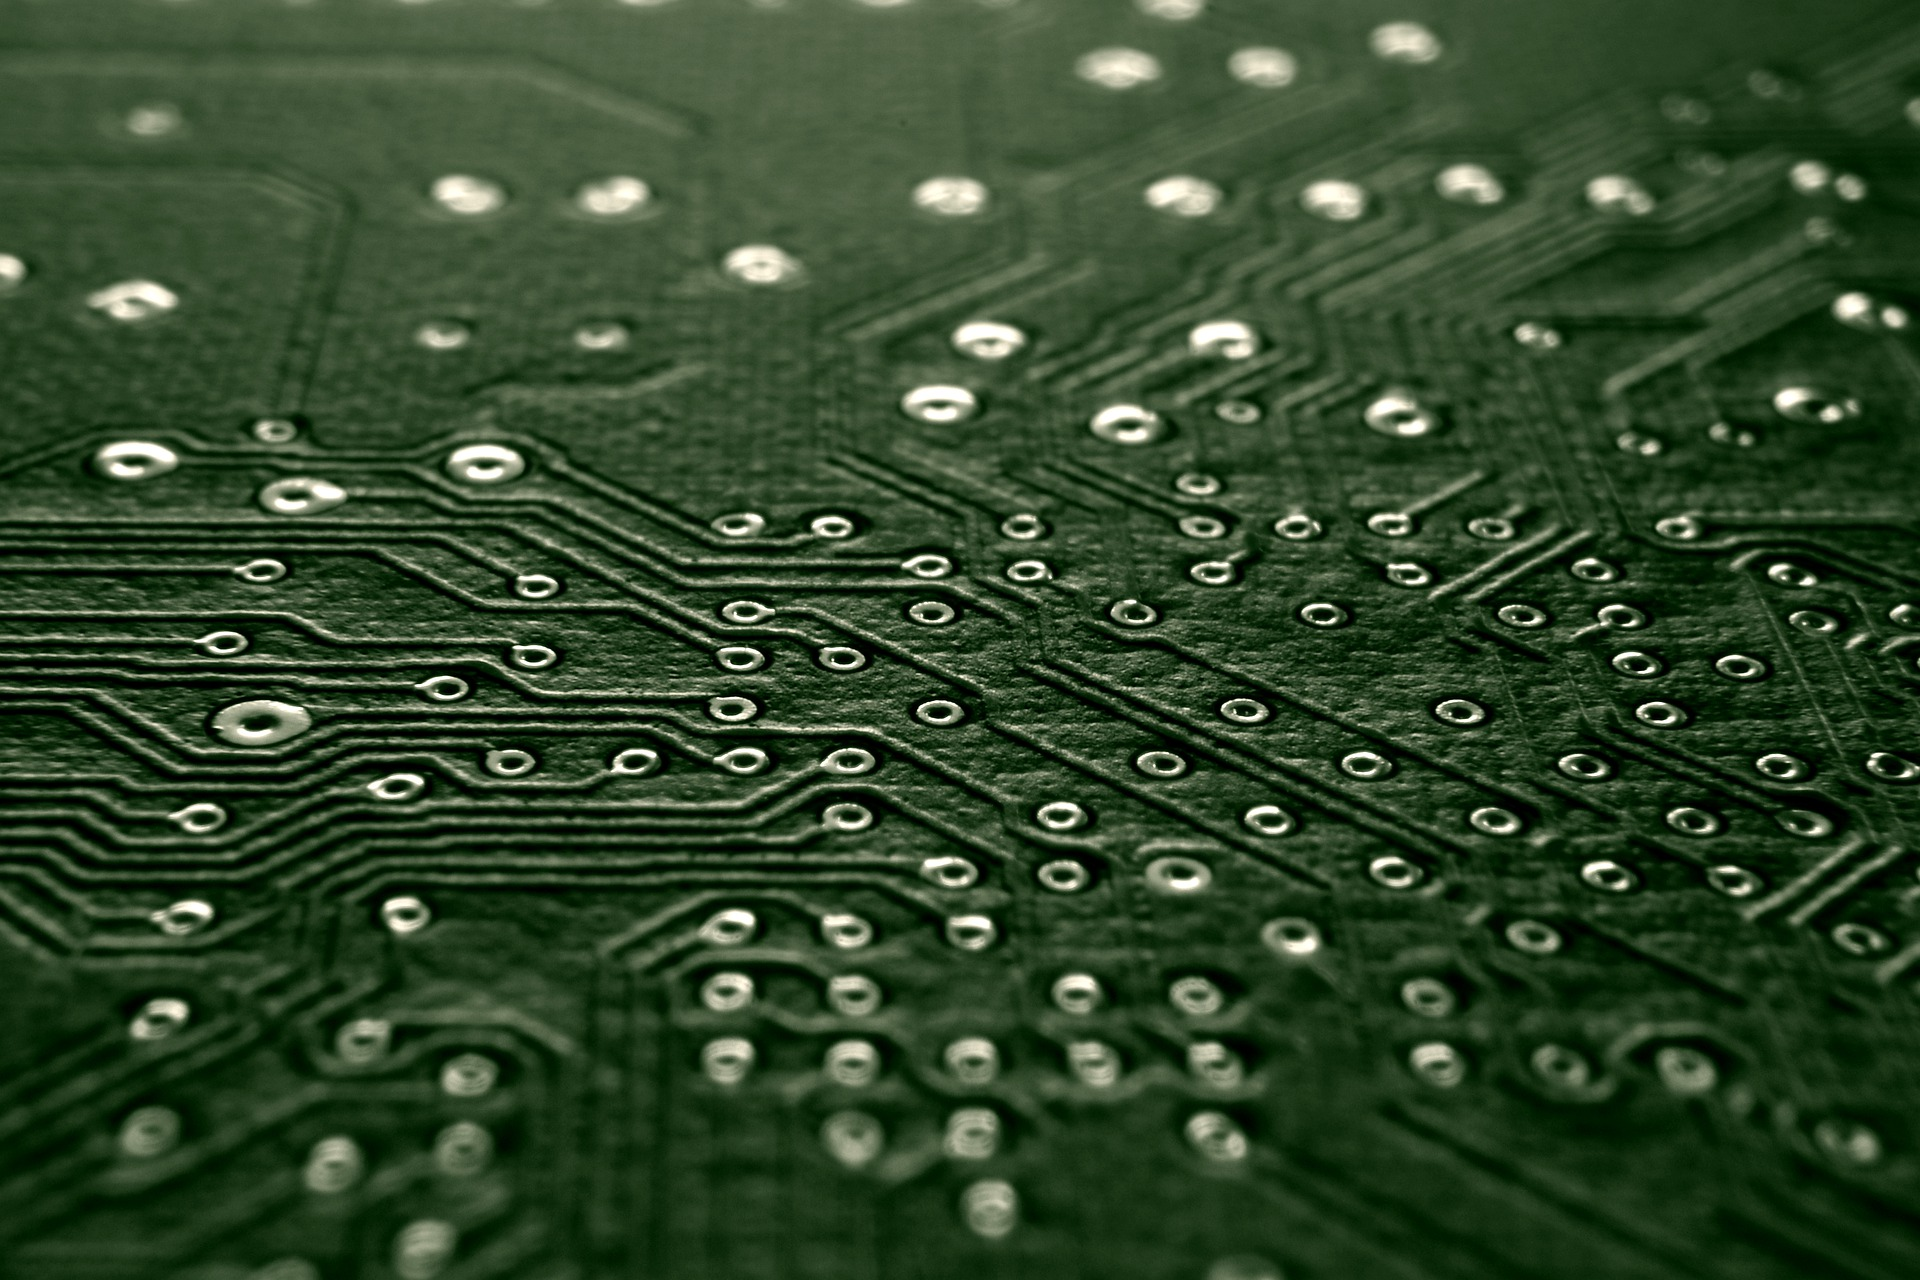
\includegraphics[scale=0.5]{computer-4491980_1920.jpg}
\centering
\vspace{2cm} \\

\textbf{Referencias} \vspace{1cm} \\
1 https://sites.google.com/site/sisoper1/home/gestion-de-memoria#:~:text=La%20parte%20del%20sistema%20operativo,necesiten%20y%20liber%C3%A1ndola%20cuando%20terminen.

\end{document}
